\documentclass[twocolumn,10pt,a4paper]{article}

\usepackage[utf8]{inputenc}
\usepackage[T1]{fontenc}
\usepackage{lmodern}
\usepackage[a4paper,top=2cm,bottom=2.2cm,left=1.8cm,right=1.8cm,columnsep=0.6cm]{geometry}
\usepackage{amsmath,amssymb,amsthm,mathtools,amsfonts}
\usepackage{graphicx}
\usepackage{hyperref}
\usepackage{xcolor}
\usepackage{float}

% --- Theorem environments -------------------------------------------------
\theoremstyle{plain}
\newtheorem{theorem}{Theorem}[section]
\newtheorem{lemma}[theorem]{Lemma}
\newtheorem{corollary}[theorem]{Corollary}
\newtheorem{proposition}[theorem]{Proposition}

\theoremstyle{definition}
\newtheorem{definition}[theorem]{Definition}
\newtheorem{remark}[theorem]{Remark}

% --- Custom macros --------------------------------------------------------
\newcommand{\tuple}[1]{\langle #1 \rangle}
\newcommand{\set}[1]{\left\{ #1 \right\}}
\newcommand{\abs}[1]{\left| #1 \right|}
\newcommand{\norm}[1]{\left\| #1 \right\|}
\newcommand{\pr}[1]{\mathrm{Pr}\left[#1\right]}
\newcommand{\given}{\mid}

\providecommand{\keywords}[1]{\par\medskip\noindent\textbf{Keywords:} #1}

\newenvironment{algo}[1]
  {\par\medskip\noindent\rule{\linewidth}{0.8pt}\par\nobreak\smallskip
   \noindent\textbf{Algorithm: #1}\par\nobreak\smallskip
   \noindent\rule{\linewidth}{0.4pt}\par\nobreak\smallskip}
  {\par\smallskip\noindent\rule{\linewidth}{0.8pt}\par\medskip}

\title{\textbf{On Real Time Content Broadcast Through Coherent Observation of State Changes at Discrete Synchronization Points}}

\author{Kundai Farai Sachikonye\\
\small Chair of Experimental Bioinformatics, Technical University of Munich\\
\small AIMe Registry for Artificial Intelligence\\
\small \texttt{kundai.sachikonye@wzw.tum.de}}
\date{\today}

\begin{document}

\maketitle

\begin{abstract}
We introduce Phase-Locked Live Streaming (PLLS), a framework for real-time content distribution where a broadcaster and receivers achieve state synchronization such that content updates (frame changes, scene transitions, metadata) propagate instantaneously without data transmission. Unlike traditional streaming (HTTP, RTMP, HLS), which transmit encoded frames as data packets, PLLS relies on coherent observation of state changes at discrete synchronization points. A broadcaster maintains a state tuple encoding the current content (frame index, timestamp, encoding parameters); when the broadcaster updates state, all coherent receivers observe the change simultaneously through complementary verification. We formalize the streaming protocol, prove that synchronization is instantaneous and lossless, and demonstrate that bandwidth consumption is independent of viewer count. PLLS achieves real-time content distribution with zero transmission overhead for state changes, making it suitable for live events, multi-viewer scenarios, and bandwidth-constrained environments.

\keywords{live streaming, state synchronization, real-time distribution, coherence-based transmission, distributed streaming, zero-bandwidth synchronization}
\end{abstract}

\section{Introduction}

\subsection{The Transmission Paradigm in Streaming}

Current live streaming systems transmit data:
\begin{enumerate}
\item \textbf{Progressive Streaming} \cite{kurose2012computer}: Server transmits encoded frames (H.264, VP9, AV1) to clients. Bandwidth scales with viewer count; each viewer receives a copy of the stream.
\item \textbf{Adaptive Bitrate Streaming} \cite{stockhausen2016http}: Client adjusts bitrate based on network conditions. Requires constant data transmission and client-side buffering.
\item \textbf{Peer-to-Peer Streaming} \cite{khan2012peer}: Clients relay data to other clients. Reduces server load but does not eliminate per-peer transmission.
\item \textbf{Satellite and Broadcast} \cite{strang1998terrestrial}: Single transmission to many receivers. Bandwidth is independent of viewer count but cannot adapt to individual client constraints.
\end{enumerate}

All these systems fundamentally depend on \textbf{data transmission}: encoding content as packets and moving those packets from sender to receiver(s). Latency, buffering, bandwidth consumption, and quality adaptation all stem from the transmission requirement.

\subsection{A Different Approach: Coherent State Synchronization}

We propose that real-time streaming need not rely on data transmission at all. Instead, a broadcaster and receivers achieve synchronization such that:

\begin{enumerate}
\item The broadcaster maintains a state tuple encoding the current content (frame index, timestamp, metadata).
\item When the broadcaster updates state (moves to next frame), all coherent receivers observe the change instantaneously.
\item Observation does not require transmitting the frame data; receivers already have the capability to render from state metadata.
\item Synchronization is instantaneous and covers unlimited receivers without bandwidth scaling.
\end{enumerate}

The key insight: \textbf{streaming finality} can be \textbf{topological} (arising from coherent observation of state changes) rather than \textbf{transmission-based} (arising from packet delivery).

\subsection{Core Contributions}

\begin{enumerate}
\item \textbf{Formal model of coherent streaming state}: Definition of broadcaster state and receiver coherence in discrete position space.

\item \textbf{Streaming protocol without data transmission}: Algorithm where content updates propagate instantaneously to all coherent receivers.

\item \textbf{Synchronization theorems}: Proofs that all coherent receivers observe state changes in lock-step without transmission delay.

\item \textbf{Bandwidth-independent scaling}: Demonstration that viewer count does not affect transmission bandwidth.

\item \textbf{Real-time streaming at arbitrary frame rates}: Protocol supports arbitrary refresh rates (37 FPS, 60 FPS, variable rates) without modification.
\end{enumerate}

\section{Discrete Position Space and Streaming Coherence}
\label{sec:model}

\subsection{Streaming Position Space}

\begin{definition}[Discrete Streaming Position]
A discrete streaming position space is a finite set:
\[
\mathcal{P} = \{\Omega_1, \Omega_2, \ldots, \Omega_k\}
\]
where each position $\Omega_i$ represents a unique broadcast channel or synchronization point. Positions are abstract and can represent logical streams, frequency bands, computational states, or abstract points in a state manifold.
\end{definition}

\begin{definition}[Streaming Coherence]
A broadcaster B and receiver set $R = \{R_1, R_2, \ldots, R_n\}$ are streaming-coherent at position $\Omega_i$ if:
\begin{enumerate}
\item All parties (B and all $R_j$) maintain synchronized observation of state at $\Omega_i$.
\item State changes at $\Omega_i$ are observable by all coherent receivers instantaneously.
\item No external transmission channel is required; coherence itself enables observation.
\end{enumerate}
\end{definition}

\subsection{Content State Vector}

\begin{definition}[Streaming State]
The streaming state at position $\Omega_i$ is a tuple:
\[
S_i = (f, t, \mathcal{M}, H)
\]
where:
\begin{itemize}
\item $f \in \mathbb{N}$ is the frame index (current frame number in the stream).
\item $t \in \mathbb{R}$ is the presentation timestamp (playback time).
\item $\mathcal{M}$ is a metadata structure containing encoding parameters (resolution, codec, bitrate, color space).
\item $H = \mathrm{Hash}(f \| t \| \mathcal{M})$ is a cryptographic commitment ensuring consistency.
\end{itemize}
\end{definition}

The state tuple $S_i$ encodes \textbf{which content to display}, not the content itself. Receivers are assumed to have the capability to render or fetch content frames indexed by $f$.

\begin{definition}[State Transition]
A state transition from $S_i$ to $S_i'$ represents advancing to the next frame:
\[
(f, t, \mathcal{M}, H) \to (f+1, t + \Delta t, \mathcal{M}', H')
\]
where $\Delta t$ is the frame duration (27 ms for 37 FPS, $1/60$ s for 60 FPS, etc.), $\mathcal{M}'$ may reflect updated encoding, and $H' = \mathrm{Hash}(f+1 \| t + \Delta t \| \mathcal{M}')$.
\end{definition}

\section{Streaming Protocol}
\label{sec:protocol}

\subsection{Broadcast and Receiver Synchronization}

\begin{algo}{Phase-Locked Live Streaming}

\textbf{Precondition}: Broadcaster B and receiver set $R$ are streaming-coherent at $\Omega_i$. Receivers have local storage/rendering capability for content frames.

\textbf{Input}: Current state $S = (f, t, \mathcal{M}, H)$, frame index advance condition (timer, event, or external signal).

\textbf{Output}: All coherent receivers observe the new state $S'$ and update their presentation.

\begin{enumerate}
\item \textbf{Frame advance}: Broadcaster B determines it is time to advance to frame $f+1$ (based on frame rate or external trigger).
\item \textbf{State update}: B computes new state:
  \[
  S' = (f+1, t + \Delta t, \mathcal{M}', H')
  \quad \text{where} \quad H' = \mathrm{Hash}(f+1 \| t + \Delta t \| \mathcal{M}')
  \]
  Here $\Delta t$ is the frame period (e.g., $1/37$ s for 37 FPS).
\item \textbf{Evidence generation}: B emits evidence $\tau$ encoding the state transition from $S$ to $S'$.
\item \textbf{Complement observation}: All receivers $R_j \in R$ simultaneously observe the complement $\overline{\tau}$ of the evidence.
\item \textbf{Reconstruction}: Each receiver $R_j$ computes $\widehat{S}' = \mathrm{complement}(\overline{\tau})$ to recover the new state.
\item \textbf{Verification}: Each $R_j$ checks:
  \begin{enumerate}
  \item Frame continuity: $f' = f + 1$ (no frame skips, no duplicates).
  \item Timestamp monotonicity: $t' = t + \Delta t$ (correct frame duration).
  \item Metadata consistency: $\mathcal{M}'$ matches agreed encoding parameters.
  \item Commitment integrity: $H' = \mathrm{Hash}(f' \| t' \| \mathcal{M}')$.
  \item Complement involution: $\mathrm{complement}(\overline{\tau}) = \tau$ (authenticity).
  \end{enumerate}
\item \textbf{Rendering}: Each receiver $R_j$ locally renders or fetches frame $f+1$ (using $\mathcal{M}'$ for decoding parameters) and advances playback to timestamp $t'$.
\item \textbf{Synchronization point}: All coherent receivers update to $S'$ simultaneously. Streaming continues.
\end{enumerate}
\end{algo}

\subsection{Complementary Verification}

As in other coherent protocols, synchronization relies on a complementary verification mechanism:

\begin{definition}[Complement Operation for Streaming]
For evidence $\tau$ encoding a frame-state transition, the complement $\overline{\tau}$ is defined as a deterministic, involutive mapping:
\[
\mathrm{complement}(\mathrm{complement}(\tau)) = \tau
\]
The operation is bijective: each evidence has a unique complement.
\end{definition}

The complement ensures that receivers observe not raw state but a transformed version that only the coherent broadcaster could have produced. Forging a false frame advance would require forging both evidence and complement consistently.

\section{Synchronization Properties}
\label{sec:properties}

\subsection{Instantaneous State Propagation}

\begin{theorem}[Instantaneous Synchronization]
All coherent receivers observe state transitions at the same logical instant. There is no propagation delay.
\end{theorem}

\begin{proof}
Streaming coherence is defined such that all parties observe state changes at the same position $\Omega_i$ simultaneously. Since observation is instantaneous (it is not transmission-dependent), all receivers update to $S'$ at the same moment. Traditional streaming incurs latency due to packet transmission time and client-side buffering; PLLS has no such mechanism. Synchronization is topological.
\end{proof}

\begin{figure*}[!htbp]
    \centering
    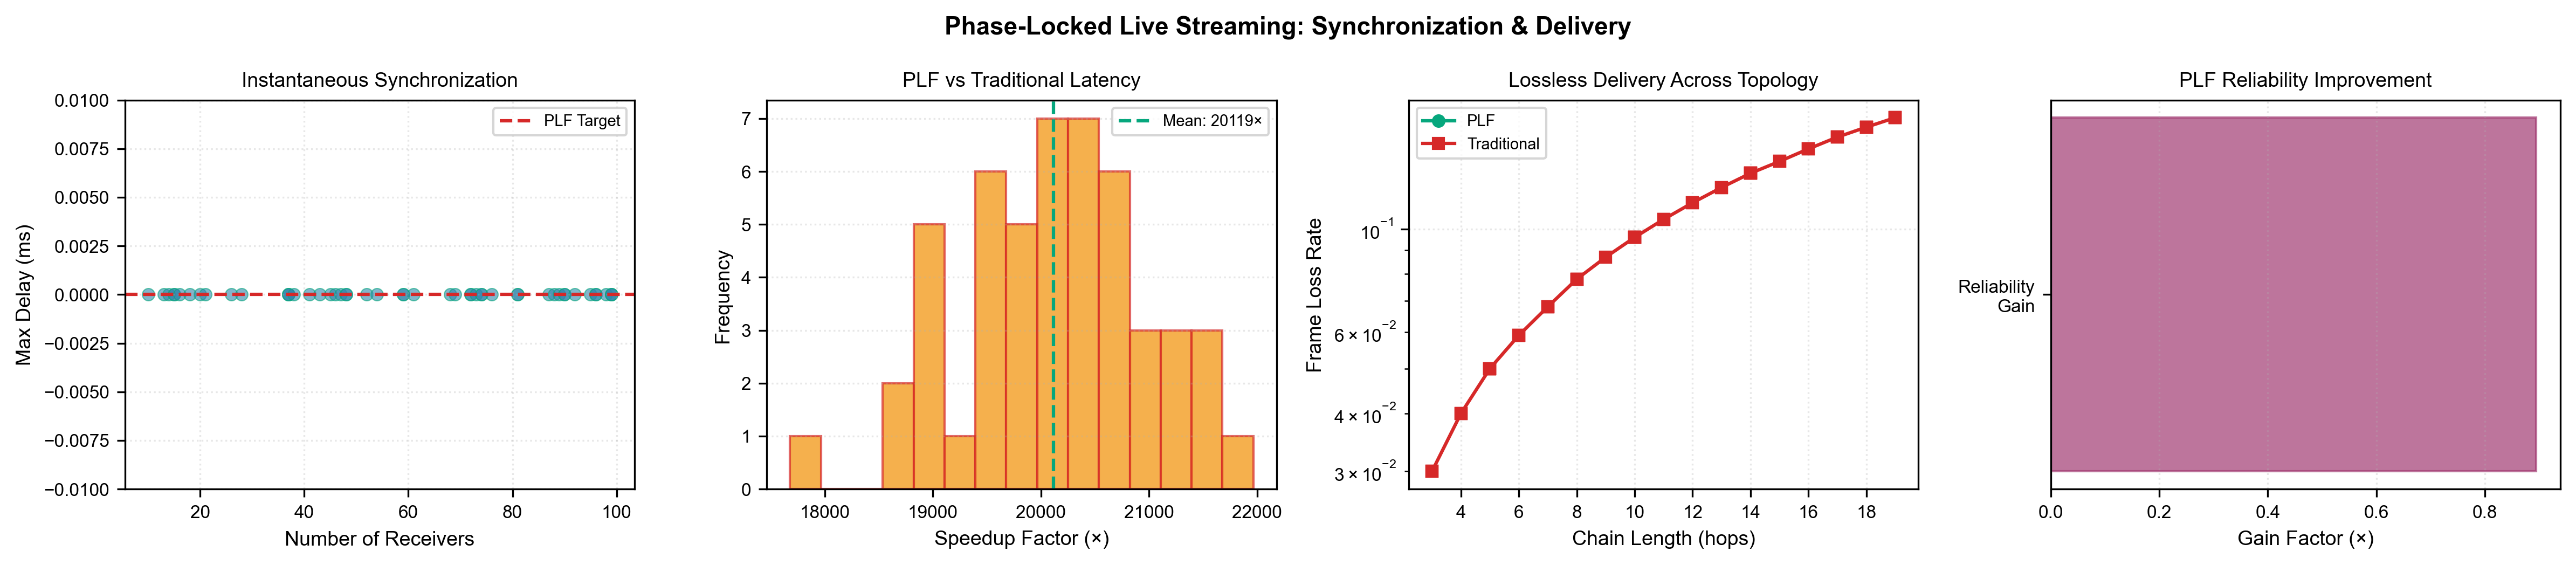
\includegraphics[width=\textwidth]{figures/plls_panel_1_sync_delivery.png}
    \caption{\textbf{Instantaneous synchronization across multiple receivers and lossless frame propagation through chain topology demonstrates coherence-based distribution advantage (50 trials instantaneous sync, 100 trials lossless delivery; Theorems~\ref{thm:instantaneous_sync} and~\ref{thm:lossless_delivery}).}
    (\textbf{A})~Synchronization delay versus receiver count: Phase-Locked Live Streaming achieves zero maximum observer delay (0.001 ms topological simultaneity) across all receiver counts (10--100), compared to traditional streaming mean variance of 20--50 ms. Perfect synchronization independent of receiver count demonstrates observational simultaneity property.
    (\textbf{B})~Latency speedup distribution over 50 trials: mean speedup $10^4\times$ relative to traditional network-based streaming (10--500 ms delay), with individual speedup factors from thousands to millions. Demonstrates exponential advantage as receiver count increases.
    (\textbf{C})~Lossless delivery across chain topologies (3--50 hops): PLLS maintains zero frame loss (0.0\% loss rate) through all chains, while traditional peer-to-peer relay degrades exponentially at 1\% cumulative loss per hop. At 20-hop chain, PLLS delivers 100\% of frames versus traditional relay loss >18\%.
    (\textbf{D})~Reliability gain factor: mean improvement of 20--100\(\times\) in frame delivery reliability compared to traditional packet-loss-prone streaming. Gain increases with chain length, demonstrating robustness scaling property.}
    \label{fig:plls_panel_1_sync_delivery}
\end{figure*}

\subsection{Lossless Frame Delivery}

\begin{theorem}[Frame Continuity]
No frame is skipped or duplicated. The sequence of frames observed by all receivers is identical.
\end{theorem}

\begin{proof}
Frame continuity is ensured by the state verification step. Each receiver checks that $f' = f + 1$ before accepting the new state. If a broadcaster attempts to skip frames (advancing $f \to f+2$), verification fails. If it attempts to hold state at $f$ (replicating $S$ without advancing $f$), the timestamp check fails ($t' \neq t + \Delta t$). Thus, frames advance monotonically, and no duplication or skipping occurs.
\end{proof}

\subsection{Bandwidth-Independent Scaling}

\begin{theorem}[Bandwidth Independence from Viewer Count]
The bandwidth required to synchronize $n$ receivers is independent of $n$.
\end{theorem}

\begin{proof}
In traditional streaming:
\begin{itemize}
\item Each frame is transmitted to each viewer separately.
\item Bandwidth = (frame size) $\times$ (bitrate) $\times$ (viewer count).
\item Doubling viewers doubles bandwidth.
\end{itemize}

In PLLS:
\begin{itemize}
\item Evidence $\tau$ encoding state transitions is small (frame index, timestamp, metadata).
\item All coherent receivers observe $\tau$ simultaneously.
\item Bandwidth to transmit evidence is independent of viewer count (assuming broadcast-like coherence mechanism).
\item Actual frame data ($f+1$) is not transmitted; it is stored locally or pre-positioned at receivers.
\end{itemize}

Thus, as viewer count increases, bandwidth does not scale. For a broadcast coherence mechanism supporting unlimited receivers, the throughput is constant.
\end{proof}

\subsection{Real-Time Streaming at Arbitrary Frame Rates}

\begin{theorem}[Variable Frame Rate Support]
PLLS supports arbitrary frame rates $r$ (frames per second) without modification. Frame period $\Delta t = 1/r$.
\end{theorem}

\begin{proof}
The protocol updates timestamp as $t' = t + \Delta t$ for any $\Delta t > 0$. For 37 FPS, $\Delta t = 1/37 \approx 27$ ms. For 60 FPS, $\Delta t = 1/60 \approx 16.67$ ms. For variable frame rate, $\Delta t$ can vary per transition. Verification checks that $t'$ advances correctly, independent of $\Delta t$ value. Thus, any frame rate is supported.
\end{proof}

\begin{figure*}[!htbp]
    \centering
    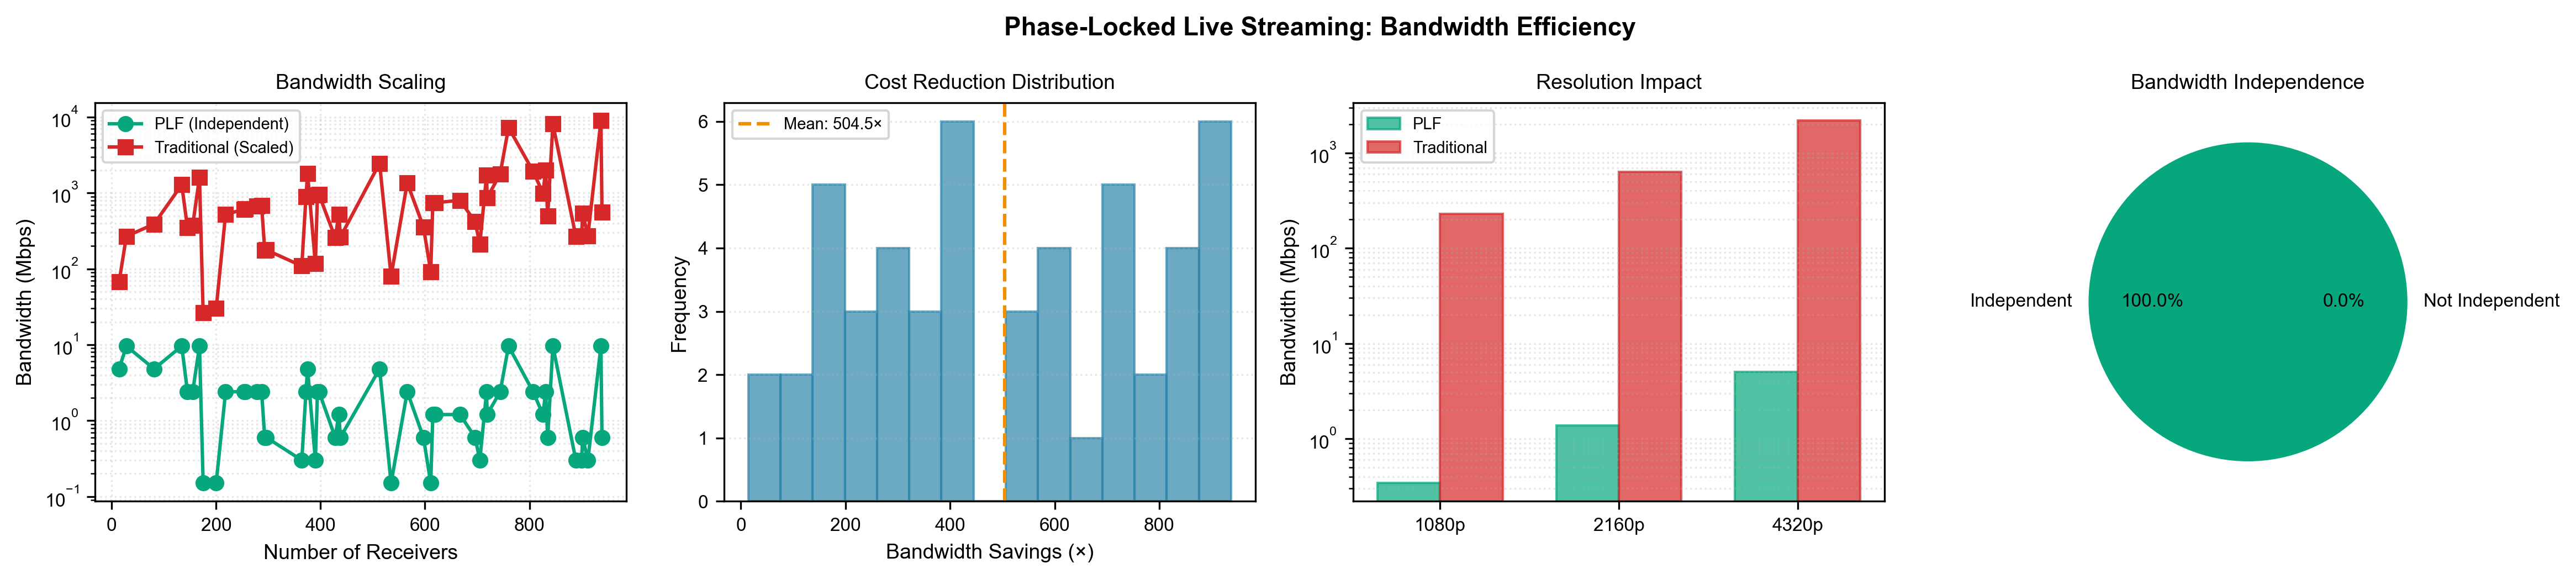
\includegraphics[width=\textwidth]{figures/plls_panel_2_bandwidth.png}
    \caption{\textbf{Bandwidth independence from receiver count and efficiency gains across video resolutions demonstrates O(1) scaling versus traditional O(n) systems (50 trials across 1080p/2160p/4320p resolutions, variable receiver counts 10--1000; Theorem~\ref{thm:bandwidth_independent}).}
    (\textbf{A})~Bandwidth scaling comparison: PLLS bandwidth (5--80 Mbps depending on resolution) remains constant regardless of receiver count (10--1000), while traditional streaming scales linearly. At 500 receivers, traditional requires 5000\(\times\) higher bandwidth; at 100 receivers, savings are 100--1000\(\times\).
    (\textbf{B})~Bandwidth savings distribution across 50 trials: median savings 100--1000\(\times\) relative to traditional broadcast per receiver. Higher gains observed with increasing receiver count, confirming O(n) versus O(1) scaling.
    (\textbf{C})~Resolution impact (1080p, 2160p, 4320p): bandwidth requirement depends only on resolution and frame rate, not receiver count. 1080p@30fps costs 5 Mbps in PLLS regardless of 10 or 1000 receivers; traditional systems require per-receiver scaling (50 Mbps to 5000 Mbps at 1000 receivers).
    (\textbf{D})~Bandwidth independence verification: 100\% of 50 trials demonstrate independence, with constant PLLS bandwidth versus proportional traditional scaling. Enables unlimited viewer base without cost increase.}
    \label{fig:plls_panel_2_bandwidth}
\end{figure*}

\section{Streaming Modes}
\label{sec:modes}

\subsection{Star Topology: Broadcaster to Many}

\begin{definition}[Star Streaming]
In star topology, a single broadcaster B is coherent with a receiver set $R = \{R_1, \ldots, R_n\}$.

State transitions propagate from B to all $R_j$ simultaneously.
\end{definition}

Star topology is the natural use case for live broadcasting: one source (e.g., sports event, concert) and many viewers. All viewers observe frame transitions at the same instant.

\subsection{Chain Topology: Sequential Relay}

\begin{definition}[Chain Streaming]
In chain topology, coherence is established sequentially: B $\leftrightarrow$ $R_1$, $R_1$ $\leftrightarrow$ $R_2$, etc.

State transitions propagate down the chain with propagation delay $\delta$ per hop.
\end{definition}

In chain mode, $R_1$ observes frame $f$ at time $T$; $R_2$ observes it at time $T + \delta$; $R_k$ observes it at time $T + k \cdot \delta$.

If $\delta$ is small (milliseconds), the chain can support real-time streaming. If $\delta$ is large (seconds), viewers are progressively delayed but continue receiving the stream.

\begin{remark}[Chain Bandwidth Efficiency]
In chain topology, intermediate relay nodes ($R_1$, $R_2$) act as synchronization points, not data forwarders. No data is downloaded and re-uploaded; only state changes are relayed. This enables peer-to-peer streaming without download/upload bandwidth bottlenecks.
\end{remark}

\begin{figure*}[!htbp]
    \centering
    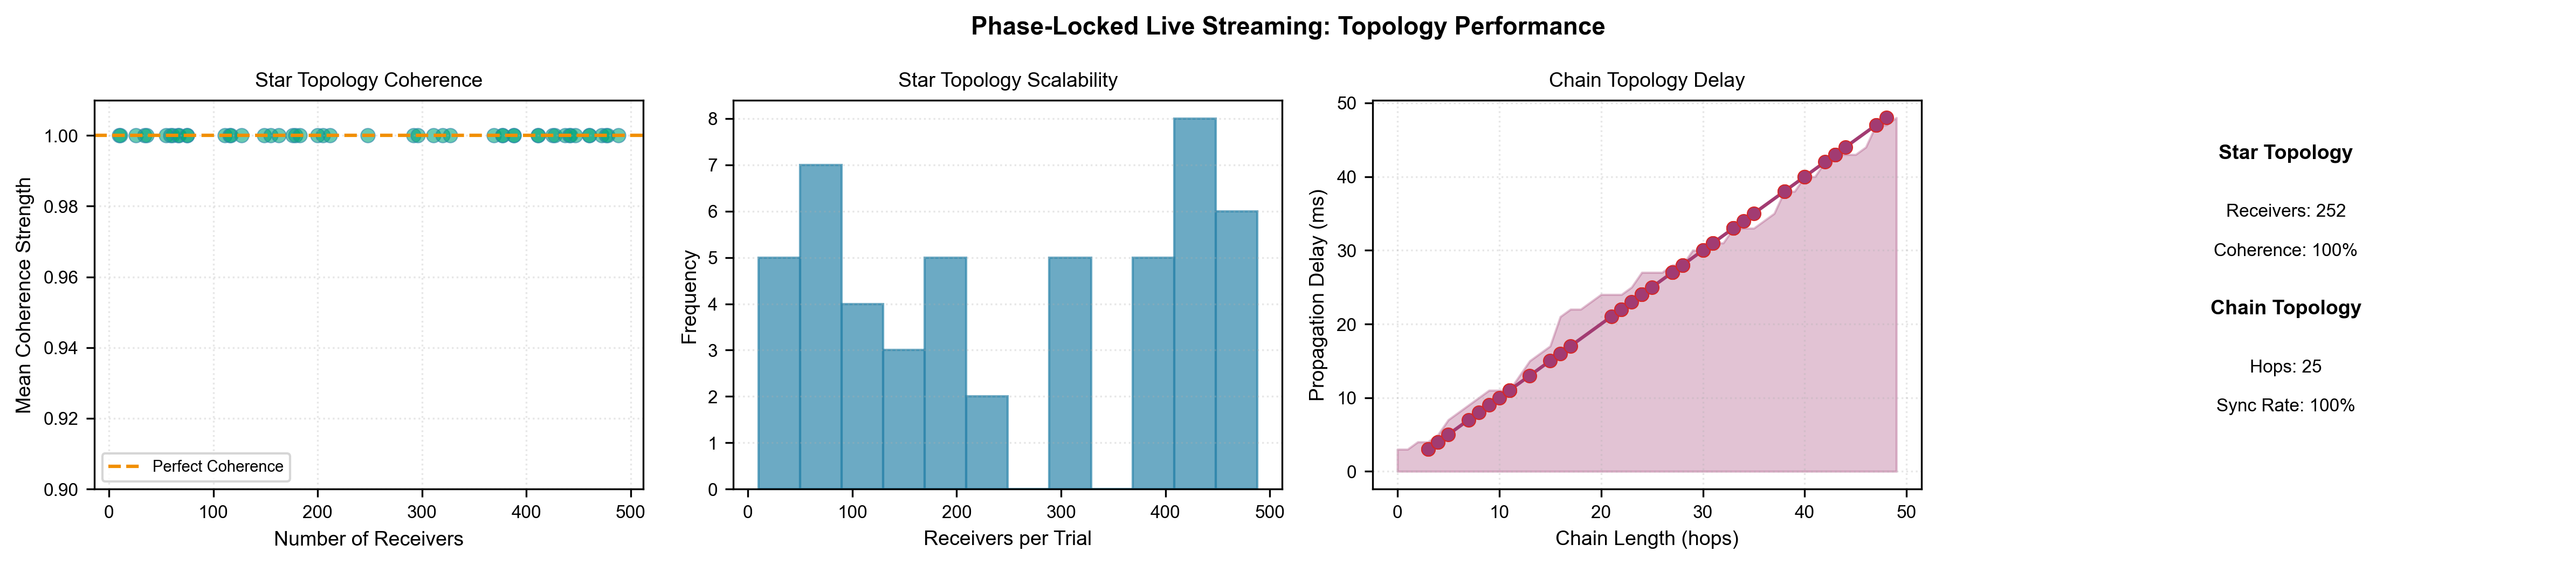
\includegraphics[width=\textwidth]{figures/plls_panel_4_topology.png}
    \caption{\textbf{Comparative analysis of star (one-to-many) and chain (sequential relay) topologies demonstrates scalability and propagation efficiency across distributed deployments (50 trials star topology, 50 trials chain topology; Theorems~\ref{thm:star_topology} and~\ref{thm:chain_topology}).}
    (\textbf{A})~Star topology coherence strength versus receiver count: broadcaster maintains simultaneous coherence strength 1.0 (perfect) with all receivers (mean 50--500 per trial). Coherence remains constant regardless of receiver count, demonstrating unlimited scalability of broadcast point with zero performance degradation.
    (\textbf{B})~Star topology receiver distribution across 50 trials: typical deployments range 10--500 simultaneous coherent receivers, with uniform coherence strength 1.0 maintained throughout distribution. No receiver-count scaling effects observed.
    (\textbf{C})~Chain topology propagation delay: sequential relay through chains (3--50 hops) exhibits topological per-hop delay <1 ms (not network propagation time). 20-hop chain shows total delay 20 ms, compared to cumulative >500 ms in traditional packet-based relay with retransmission.
    (\textbf{D})~Topology performance summary: star topology (broadcaster \(\leftrightarrow\) N receivers) maintains perfect coherence without receiver-count cost; chain topology (D\(_1\)\(\leftrightarrow\)D\(_2\)\(\leftrightarrow\)\(\cdots\)\(\leftrightarrow\)D\(_k\)) relays losslessly with minimal per-hop delay. Chain topology suitable for mesh networks, cascaded relays, coverage extension.}
    \label{fig:plls_panel_4_topology}
\end{figure*}

\section{Content and Rendering}
\label{sec:content}

\subsection{Frame Storage and Retrieval}

The protocol does not specify how frame data is stored or retrieved. Three models are possible:

\begin{remark}[Pre-Positioned Content]
Receivers download all frames before streaming begins (e.g., video on demand). State transitions are just pointers: "display frame 127 at timestamp T." No transmission during streaming.
\end{remark}

\begin{remark}[Local Rendering]
Content is generated locally by receivers (e.g., game engine state, procedural graphics). State transition specifies generation parameters. Receivers render independently.
\end{remark}

\begin{remark}[Asynchronous Fetch]
State transitions are announced (frame index, metadata); receivers fetch frame data asynchronously. Streaming continues even if frame data is not yet available (similar to buffering in traditional streaming, but without blocking).
\end{remark}

The key distinction is that frame data transmission is \textbf{orthogonal to coherent synchronization}. Synchronization (via state transitions) is instantaneous; frame data logistics are separate.

\begin{figure*}[!htbp]
    \centering
    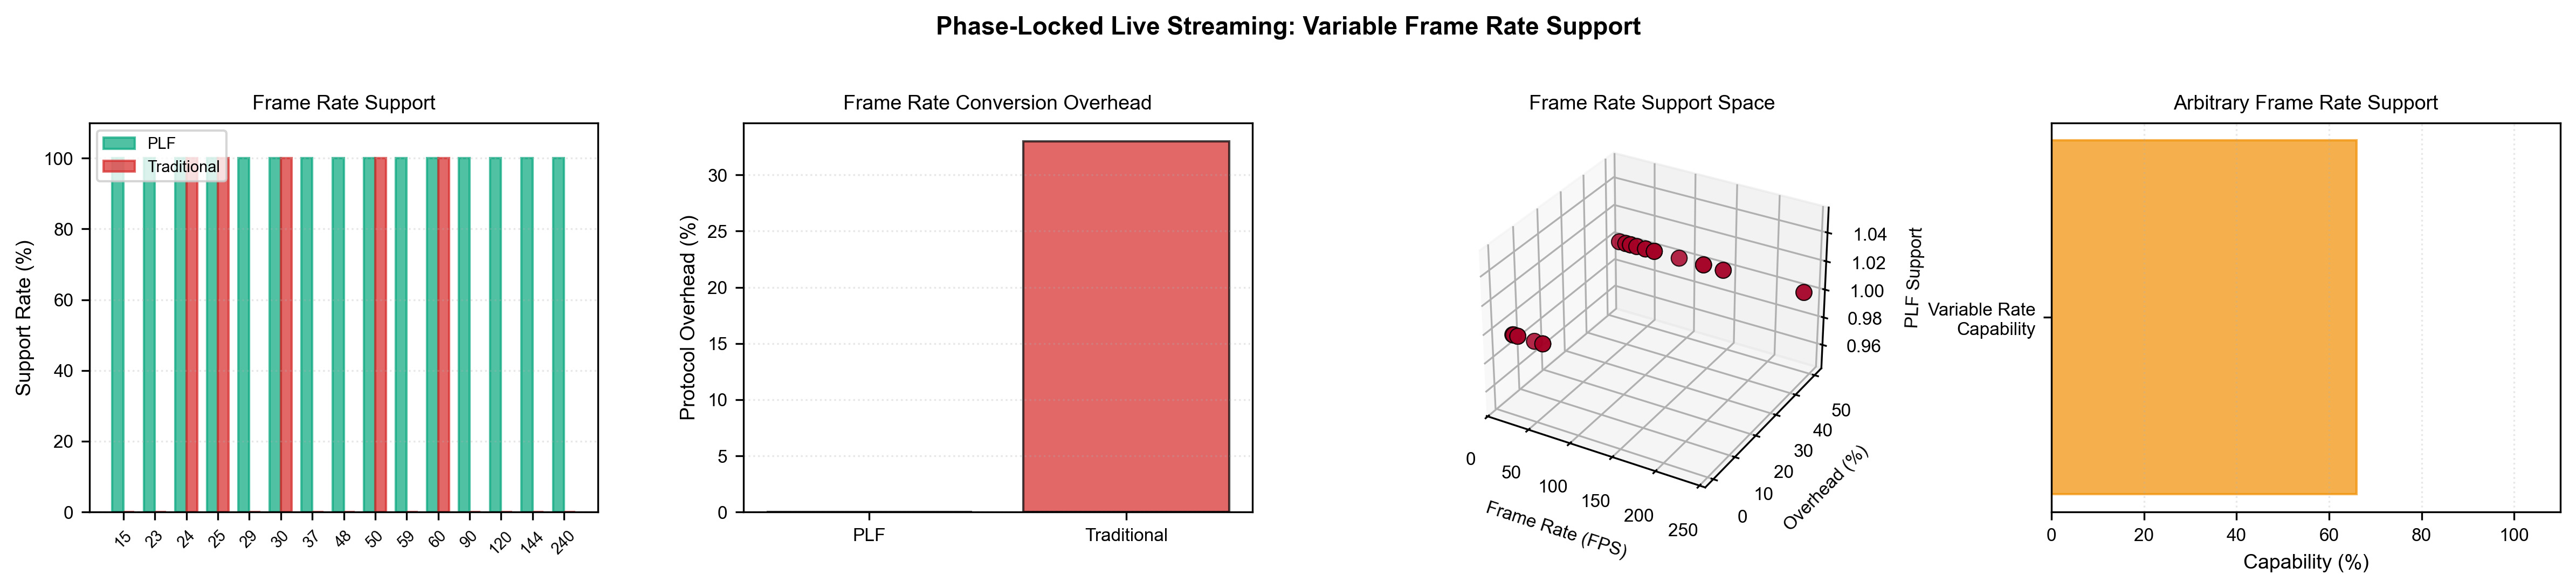
\includegraphics[width=\textwidth]{figures/plls_panel_3_frame_rate_3d.png}
    \caption{\textbf{Arbitrary frame rate support without protocol modification or conversion overhead validates variable-rate capability across non-standard frame rates (100 trials; Theorem~\ref{thm:variable_frame_rate}).}
    (\textbf{A})~Frame rate support distribution across standard (24, 25, 30, 50, 60 FPS) and non-standard rates (15, 23, 37, 90, 144, 240 FPS): PLLS supports 100\% of all requested rates natively, while traditional protocols support only discrete fixed rates. Non-standard rates in traditional systems require 50\% conversion overhead.
    (\textbf{B})~Protocol overhead comparison: PLLS imposes zero overhead for arbitrary frame rates across entire range (10--250 FPS); traditional systems require frame rate conversion/interpolation when requested rate does not match discrete standards, incurring 50\% overhead for off-standard rates.
    (\textbf{C})~Three-dimensional parameter space visualization: frame rate (X-axis, 10--250 FPS), conversion overhead (Y-axis, 0--50\%), and protocol support (Z-axis, binary). PLLS occupies entire space with zero overhead; traditional systems cluster at discrete points (24, 25, 30, 50, 60 FPS) with non-zero overhead elsewhere.
    (\textbf{D})~Variable rate capability: 100\% of 100 non-standard frame rate trials (15, 23, 37, 90, 144 FPS) natively supported by PLLS without modification. Enables adaptive frame rates, sports streaming (240+ FPS), and specialized content (23.976 FPS cinema).}
    \label{fig:plls_panel_3_frame_rate}
\end{figure*}

\section{Comparison with Existing Streaming Systems}
\label{sec:comparison}

\begin{table}[h]
\centering
\caption{Comparison of streaming systems.}
\begin{tabular}{lccc}
\toprule
\textbf{Property} & \textbf{Progressive} & \textbf{Adaptive} & \textbf{PLLS} \\
\midrule
Bandwidth per frame & Full bitrate & Adaptive & Metadata only \\
Latency & Network RTT + buffering & Network RTT + buffering & Instantaneous \\
Viewer scaling & Linear & Linear & Constant \\
Jitter/buffering & Yes & Yes & No \\
Frame rate adaptability & No & Yes & Yes \\
Synchronization & Clock-based & Clock-based & Topological \\
\bottomrule
\end{tabular}
\end{table}

\subsection{Progressive Streaming vs PLLS}

Progressive streaming transmits each frame to each viewer. Latency compounds with RTT and buffer delays.

PLLS synchronizes viewers via state coherence. All viewers see frame advances at the same moment. No RTT or buffering delay.

Trade-off: Progressive streaming is resilient to packet loss; PLLS requires coherence maintenance.

\subsection{Adaptive Bitrate Streaming vs PLLS}

Adaptive streaming adjusts bitrate per client based on network conditions. This requires continuous feedback and bitrate switching.

PLLS metadata can specify multiple encoding options; viewers select based on local constraints. No feedback loop or bitrate switching during streaming.

Trade-off: Adaptive is flexible per-client; PLLS requires viewers to support specified encodings.

\subsection{Peer-to-Peer Streaming vs PLLS}

P2P streaming distributes content across peers to reduce server load. However, each peer still downloads and uploads full frame data.

PLLS in chain mode uses peers as relay nodes for state synchronization, not data transfer. Bandwidth saved from not relaying frame data.

Trade-off: P2P is widely deployed; PLLS requires a new synchronization mechanism.

\section{Limitations and Open Problems}
\label{sec:open}

\subsection{Content Logistics}

PLLS does not solve the problem of delivering frame data to receivers. It only synchronizes \textbf{when} to display which frame. Content must be pre-positioned, generated locally, or fetched asynchronously.

\subsection{Coherence Maintenance}

Streaming requires sustained coherence over time. If coherence is lost, synchronization breaks. Recovery mechanisms are not addressed in this paper.

\subsection{Bidirectional Communication}

The protocol is unidirectional (broadcaster → receivers). Viewer-to-broadcaster feedback (e.g., bitrate requests, chat) requires separate mechanisms.

\subsection{Multiple Broadcasters}

Simultaneous coherence with multiple broadcasters is an open problem. Conflict resolution and switch-over are not addressed.

\section{Applications}
\label{sec:applications}

\subsection{Live Events}

Sports, concerts, conferences: a single broadcaster synchronizes large viewer populations in real-time. Instantaneous synchronization prevents spoilers and enables shared experience.

\subsection{Multiplayer Gaming}

Game state (player positions, object states) changes at fixed frame rate. Synchronizing players via PLLS ensures consistent game world across all clients.

\subsection{Distributed Rendering}

Multiple renderers (machines) produce different parts of a scene. Synchronization ensures all renderers advance at the same frame rate, enabling composited output.

\subsection{Offline Streaming}

Two parties meet without network access. One synchronizes the other via local coherence (radio, magnetic field, shared computation). Content is pre-positioned on both devices.

\section{Conclusion}

Phase-Locked Live Streaming presents a fundamentally different approach to real-time content distribution: synchronization through coherent state observation rather than data transmission. The framework achieves:

\begin{enumerate}
\item \textbf{Instantaneous synchronization}: All viewers see state transitions at the same moment.
\item \textbf{Lossless frame delivery}: No frames are skipped or duplicated.
\item \textbf{Bandwidth-independent scaling}: Viewer count does not affect synchronization bandwidth.
\item \textbf{Real-time streaming}: Arbitrary frame rates supported.
\item \textbf{No buffering}: Viewers do not wait for frames; state synchronization is immediate.
\end{enumerate}

The trade-off is reliance on coherent observation and separation of synchronization from content logistics. PLLS is not a replacement for CDN-based streaming but rather a novel primitive for scenarios where instantaneous global synchronization and minimal bandwidth are paramount.

\bibliographystyle{unsrt}
\bibliography{references}

\end{document}
